Algoritmos como K-Means presentan dificultades para identificar clusters cuando las distancias entre elementos de un mismo conjunto es mayor que la de elementos de conjuntos distintos.
En estos casos, puesto que K-Means busca minimizar la distancia entre los elementos dentro de un mismo cluster, producirá clusters que difieran significativamente de los grupos <<correctos>>.
Podemos observar un ejemplo en el escenario de la figura~\ref{img:kmeans-dbscan}, donde se compara el resultado de K-Means con el del algoritmo que analizamos en esta sección, conocido como \textit{DBSCAN}.

\begin{figure}[!h]
    \centering
    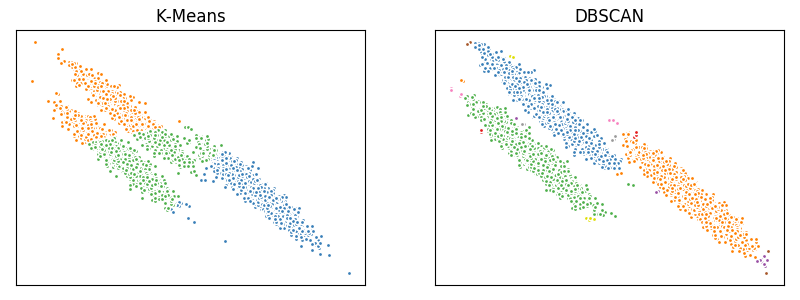
\includegraphics[width=\textwidth]{kmeans-dbscan.png}
    \caption{Resultados de los algoritmos K-Means y DBSCAN ejecutados sobre un conjunto de datos que sigue una distribución anisotrópica.}
    \label{img:kmeans-dbscan}
\end{figure}

En la imagen podemos observar asimismo el comportamiento de otro algoritmo sobre el mismo conjunto de datos.
En esta sección abordamos el algoritmo en cuestión, denominado \textit{DBSCAN}~\footnote{Siglas en inglés de \textit{Density-based spatial clustering of applications with noise}.}, que forma parte del conjunto de algoritmos de clustering basados en la densidad de los datos.

Un cluster basado en el criterio de densidad de los puntos consiste en un área densa de puntos conectados, separado de otros clusters por áreas de menor densidad.

\subsection{Densidad}\label{subsec:densidad}

El algoritmo DBSCAN define la densidad alrededor de un punto como la cantidad de puntos localizados alrededor de este en un radio, $Eps$, específico.
El propio punto es incluido en este conteo.
En la figura~\ref{img:dbscan} se puede observar gráficamente esta definición.
En este caso número de puntos alrededor de $A$ es 7.

El valor del radio es determinante en la densidad de un punto.
Si este valor es suficientemente grande, entonces todos los puntos tendrán una densidad de $n$, el número de puntos en el conjunto de datos.
En cambio, si el radio es demasiado pequeño, la densidad de todos los puntos será igual a 1.
Más adelante discutiremos algunas estrategias para la selección de valores apropiados para el radio.

\begin{figure}[!h]
    \centering
    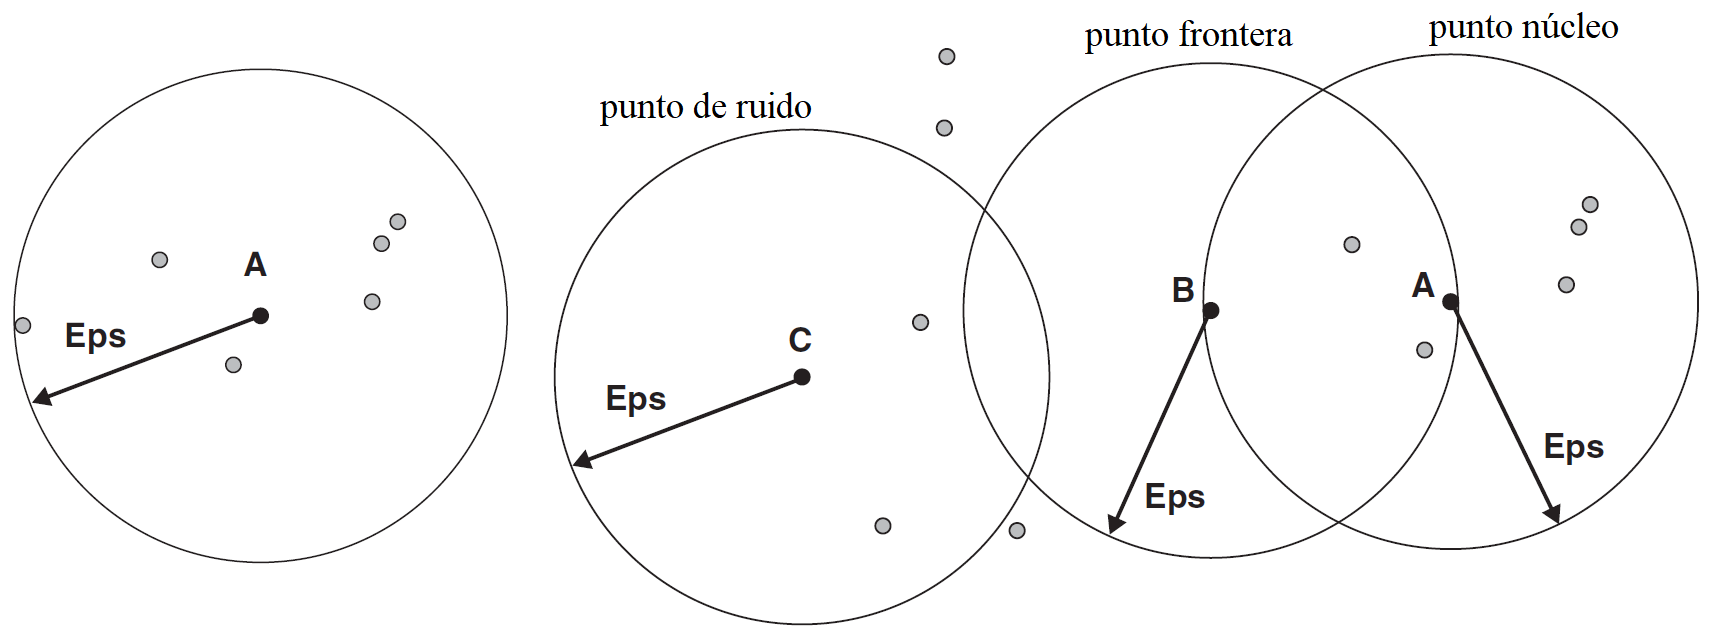
\includegraphics[width=0.8\textwidth]{dbscan.png}
    \caption{Densidad en el entorno de un punto y clasificaciones de los puntos según su densidad. (Tomado de~\cite{Tan05}.)}
    \label{img:dbscan}
\end{figure}

De acuerdo con la densidad de un punto, estos pueden ser clasificados de la siguiente forma:

\begin{itemize}
    \item \textbf{Puntos núcleo}: Constituyen puntos de la región interna de un cluster basado en densidad.
    Un punto es núcleo si el número de puntos alrededor de este (incluyéndolo) supera o iguala un valor $MinPts$, especificado por el usuario.
    En la figura~\ref{img:dbscan} los puntos identificados con la letra $A$ son núcleos para el radio $Eps$ indicado si $MinPts\leq 7$.
    \item \textbf{Puntos frontera}: Un punto frontera es aquel que no cumple el criterio de núcleo, pero que forma parte de la vecindad de al menos uno de estos.
    En la figura~\ref{img:dbscan} $B$ es un punto frontera.
    \item \textbf{Puntos de ruido}: Un punto es de ruido si no es núcleo o frontera.
    En la figura~\ref{img:dbscan} $C$ es un punto de ruido.
\end{itemize}

\subsection{Algoritmo DBSCAN}\label{subsec:DBSCAN}

A partir de las definiciones dadas de puntos núcleos, fronteras y de ruido, podemos describir el algoritmo DBSCAN del siguiente modo: Todo par de puntos núcleos cuya distancia sea no mayor que $Eps$ son asignados al mismo cluster.
De igual forma, los puntos fronteras son asignados al cluster de los puntos núcleos cuya distancia a estos sea menor o igual que $Eps$.
(En caso de estar en la vecindad de núcleos pertenecientes a clusters diferentes, un criterio específico debe ser determinado al programar el algoritmo).
Los puntos de ruido son descartados y no asignados a ningún cluster.

\begin{algorithm}
    \caption{DBSCAN}
    \label{algorithm:DBSCAN}
    Etiquetar todos los puntos como núcleo, frontera o ruido\;
    Eliminar los puntos de ruido\;
    Añadir una arista entre todo par de puntos núcleos que se encuentren a una distancia menor o igual que $Eps$\;
    Convertir cada componente conexa del grafo resultante en un cluster\;
    Asignar cada punto frontera a uno de los clusters de los puntos núcleos asociados a este\;
\end{algorithm}

\subsubsection{Complejidad espacial y temporal}

El algoritmo DBSCAN demora en ejecución un tiempo $O(n \cdot$ tiempo para encontrar puntos en una $Eps$-vecindad), donde $n$ es el número de puntos en el conjunto de datos.
En el peor caso, esta complejidad sería $O(n^2)$.
Sin embargo, el uso de determinadas estructuras de datos en espacios de pocas dimensiones, permite la recuperación eficiente de todos los puntos en un intervalo dado alrededor de un punto específico~\cite{Tan05};
en estos escenarios la complejidad puede llegar a ser $O(n\log n)$.
Los requerimientos de memoria de DBSCAN, aun en espacios de grandes dimensiones, son $O(n)$, puesto que solo es necesario mantener poca información relativa a cada punto, como puede ser el cluster al que pertenece, la clasificación, etc.
No obstante, este uso de memoria depende igualmente del comportamiento de la estructura de datos empleada para computar las vecindades.

\subsubsection{Selección de parámetros para DBSCAN}\label{subsubsec:paramsDBSCAN}

Un criterio para determinar los parámetros es mediante la observación del comportamiento de la distancia de los puntos a su $k$-ésimo vecino más cercano, que llamaremos $k$-distancia~\footnote{En la bibliografía en inglés suele nombrársele \textit{core distance}.}.
Si un punto pertenece a un cluster, entonces su $k$-distancia debe ser un valor relativamente pequeño, siempre que $k$ no sea mayor que el tamaño del cluster.
Siempre que las densidades de los clusters no difieran radicalmente, en promedio, los valores de la $k$-distancias para puntos que pertenezcan a algún cluster no mostrarán un rango de valores muy amplio.
En cambio, para puntos que no pertenezcan a ningún cluster, es decir, de ruido, este valor sí estará situado muy por encima del rango antes mencionado.
De esta forma, si tomamos todos los puntos de un conjunto de datos, los ordenamos por su $k$-distancia y estas las representamos en una gráfica (ver figura~\ref{img:dbscan-k-dist}), deberíamos obtener una imagen donde existirá un punto de inflexión que se corresponda con el valor de la $k$-distancia a partir del cual los puntos se encuentran fuera de algún cluster.
Podemos entonces tomar dicho valor como el $Eps$ adecuado para el problema en cuestión.
En cuanto al valor de $MinPts$, este sería precisamente el $k$ seleccionado para calcular las distancias, pues los puntos cuya $k$-distancia sea menor que $Eps$ serán etiquetados como núcleos, mientras los demás serán fronteras o ruido.

\begin{figure}[!h]
    \centering
    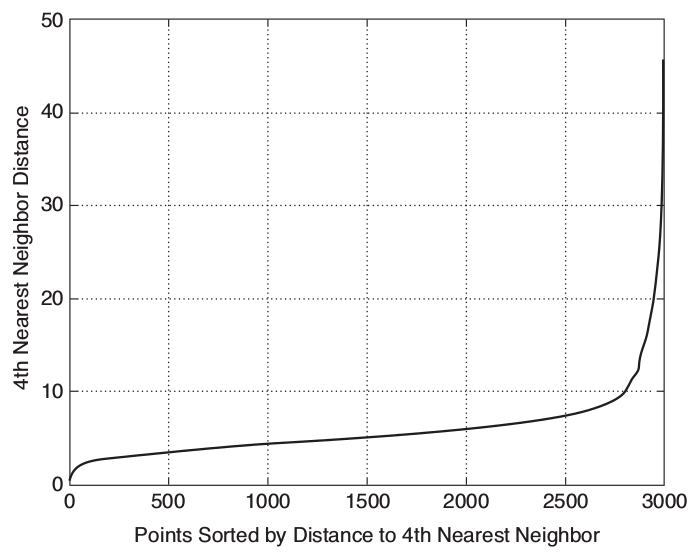
\includegraphics[width=0.5\textwidth]{dbscan-k-dist.png}
    \caption{Representación de los puntos de un conjunto de datos ordenados por su $k$-distancia ($k=4$). (Tomado de~\cite{Tan05}.)}
    \label{img:dbscan-k-dist}
\end{figure}

Es importante notar que el valor de $Eps$ resultante de este proceso dependerá del $k$ seleccionado al inicio.
Si $k$ es demasiado pequeño, algunos puntos de ruido situados muy próximos entre sí pudieran ser etiquetados incorrectamente como clusters.
Por otra parte, si $k$ es demasiado grandes, aquellos clusters cuya cantidad de elementos sea menor que $k$ no serán identificados correctamente.

Un defecto del algoritmo DBSCAN es que requiere que las densidades de los clusters (y del espacio de datos en general) muestren comportamientos semejantes.
Un ejemplo de esta afirmación podemos observarlo en la figura~\ref{img:density-issues}.
El ruido alrededor de los clusters $A$ y $B$ presenta la misma densidad que los clusters $C$ y $D$.
Si seleccionamos un $Eps$ suficientemente bajo para detectar a $C$ y $D$, sucederá entonces que $A$, $B$ y el ruido a su alrededor constituirán un mismo cluster.
En cambio si el $Eps$ es tan alto como para distinguir a $A$ y $B$ como clusters independientes, entonces los puntos que forman parte de $C$ y $D$ serán considerados ruido.

\begin{figure}[!h]
    \centering
    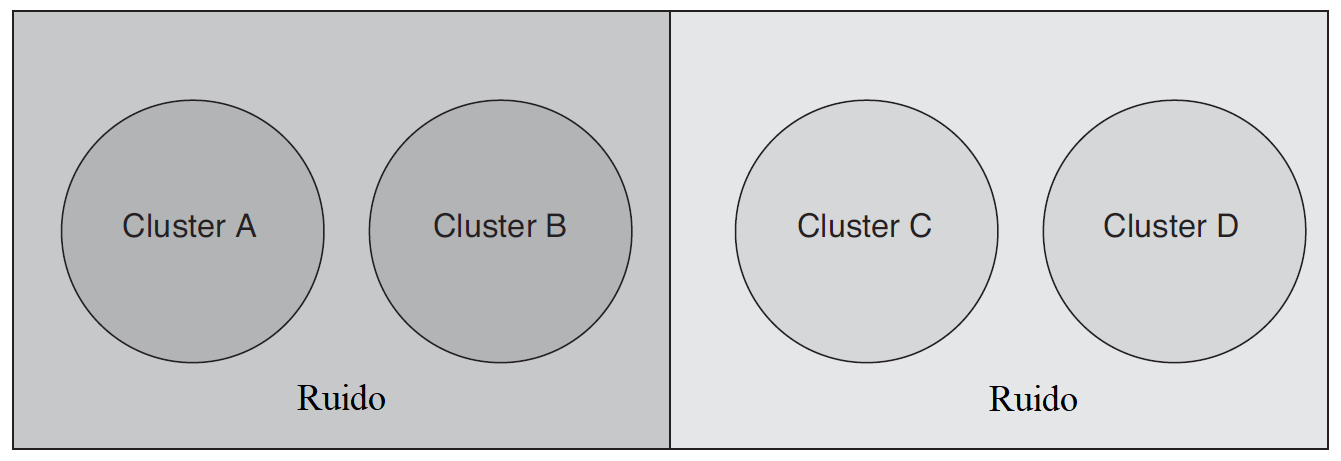
\includegraphics[width=0.8\textwidth]{density-issues.png}
    \caption{Cuatro clusters en un entorno de ruido.
    Los tonos de gris más oscuros indican mayores densidades. (Tomado de~\cite{Tan05}.)}
    \label{img:density-issues}
\end{figure}

\subsection{Algoritmo HDBSCAN}\label{subsec:HDBSCAN}

HDBSCAN~\footnote{\textit{Hierarchical DBSCAN} en inglés, o \textit{DBSCAN jerárquico} en español.} es un algoritmo creado en 2013~\cite{Campello13}, basado en la combinación del concepto de densidad con el clustering jerárquico.
Fue propuesto como solución a algunas desventajas presentes en DBSCAN y otros algoritmos de clustering, como las mencionadas en el epígrafe anterior.

La idea detrás del algoritmo consiste en usar DBSCAN convertido en algoritmo de clustering jerárquico, y luego emplear una técnica basada en el concepto de \textit{estabilidad} de un cluster para extraer los clusters a partir de la jerarquía encontrada~\cite{McInnes17}.

\begin{algorithm}
    \caption{HDBSCAN}
    \label{algorithm:HDBSCAN}
    Transformar el espacio en correspondencia con la densidad/dispersión de los puntos\;
    Computar el árbol abarcador de costo mínimo correspondiente al grafo completo ponderado por las distancias halladas\;
    Construir una jerarquía de componentes conexas (clusters)\;
    Condensar la jerarquía a partir de un tamaño mínimo para los clusters\;
    Extraer los clusters estables del árbol condensado\;
\end{algorithm}

El primer paso del algoritmo HDBSCAN busca transformar las distancias con la finalidad de evitar la sensibilidad del clustering jerárquico a los puntos de ruido en el conjunto de datos.
La nueva matriz de distancias conservará las distancias entre puntos situados en áreas densas del espacio;
mientras que asociará valores más altos a las distancias correspondientes a puntos ubicados fuera de estas.

Primero se calculan las $k$-distancias (ver página~\ref{subsubsec:paramsDBSCAN}) de cada punto $x$ del conjunto de datos: $dist_k(x)$.
A continuación, se construye la nueva matriz de distancias, empleando la función conocida como \textit{distancia de alcanzabilidad mutua}~\footnote{\textit{mutual reachability distance} en inglés.} definida por la ecuación~(\ref{eq:d_mreach}):

\begin{equation}
    \label{eq:d_mreach}
    d_{mreach}(a,b)=\max(dist_k(a), dist_k(b), dist(a,b))
\end{equation}

\noindent
donde $dist(a,b)$ es la distancia original entre los puntos $a$ y $b$.
Como mencionamos anteriormente, bajo esta nueva métrica, los puntos de regiones densas permanecen a la misma distancia, pues sus $k$-distancias tienen valores relativamente pequeños y siendo entonces su distancia entre sí quien domina en la ecuación~(\ref{eq:d_mreach}).
Lo contrario ocurre en puntos localizados en regiones esparcidas, en dichos casos se impone su $k$-distancia y por tanto son alejados del resto de los puntos a al menos dicho valor.

El uso de la distancia de alcanzabilidad mutua como alternativa a la medida de distancia tradicional mejora significativamente los resultados obtenidos al aproximar mediante una jerarquía la distribución de las densidades de los puntos del conjunto de datos~\cite{Eldridge15}.

\begin{figure}[!h]
    \centering
    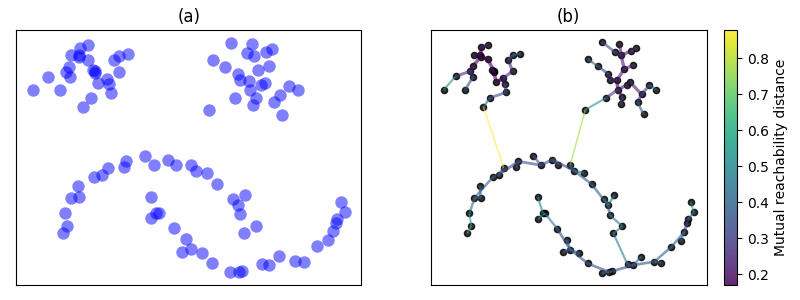
\includegraphics[width=\textwidth]{hdbscan-dataset+mst.png}
    \caption{(a) Conjunto de datos generado de forma aleatoria. (b) Árbol abarcador de costo mínimo correspondiente a la matriz de distancias de alcanzabilidad mutuas.}
    \label{img:hdbscan-dataset+mst}
\end{figure}

Una vez obtenido el árbol abarcador de costo mínimo, el siguiente paso consiste en construir una jerarquía de componentes conexas (clusters) a partir de este.
Para ello eliminamos todas las aristas del grafo y las añadimos en orden ascendente según su peso, cada componente conexa que unen constituye el cluster padre de los clusters correspondientes en la jerarquía.

\begin{figure}[!h]
    \centering
    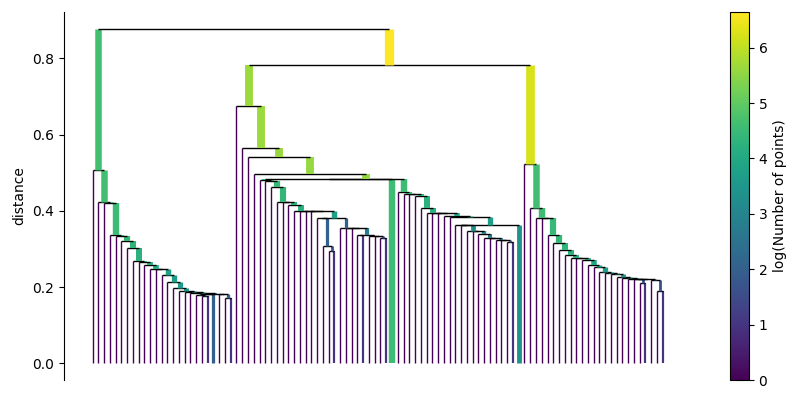
\includegraphics[width=0.8\textwidth]{hdbscan-hierarchy.png}
    \caption{Jerarquía de clusters obtenida tras el paso 3 del algoritmo HDBSCAN aplicado al conjunto de datos de la figura~\ref{img:hdbscan-dataset+mst}a.}
    \label{img:hdbscan-hierarchy}
\end{figure}

El próximo paso consiste en obtener un conjunto disjunto de clusters a partir de la jerarquía, que represente al conjunto de datos de un modo equivalente al que produce el algoritmo DBSCAN\@.
En este paso, ocurre una diferencia sustancial entre el enfoque del algoritmo DBSCAN y el de HDBSCAN\@.
Mientras el primero opta por producir una respuesta donde los parámetros $Eps$ y $MinPts$ (ver página~\ref{subsubsec:paramsDBSCAN}) determinan el nivel al que se corta el árbol de la jerarquía y los clusters que son desechados como ruido;
HDBSCAN no corta el árbol a un nivel dado, sino que selecciona los clusters a diferentes niveles, permitiendo así detectar agrupaciones de densidad variable.

El paso 4 del algoritmo <<condensa>> el árbol de la jerarquía del paso anterior, lo que permite asociar a cada nodo una mayor cantidad de información.
A menudo, mientras descendemos en la jerarquía observamos que, al dividirse un cluster, solo se separan unos pocos puntos mientras el grueso de sus elementos permanecen en el otro cluster hijo.
Si no consideramos estas divisiones donde se pierden \textit{pocos} puntos y en su lugar simplemente eliminamos tales puntos del cluster en cuestión, obtendremos una versión simplificada del árbol de la jerarquía;
donde las ramas realmente implican una división del cluster más que la eliminación de puntos de ruido.
Esta es precisamente la versión condensada de la jerarquía.
Y para lograr diferenciar entre las ramificaciones, HDBSCAN recibe un parámetro conocido como \textbf{tamaño mínimo de cluster}, que sirve como cota inferior para los clusters que son incluidos en el árbol condensado.

\begin{figure}[!h]
    \centering
    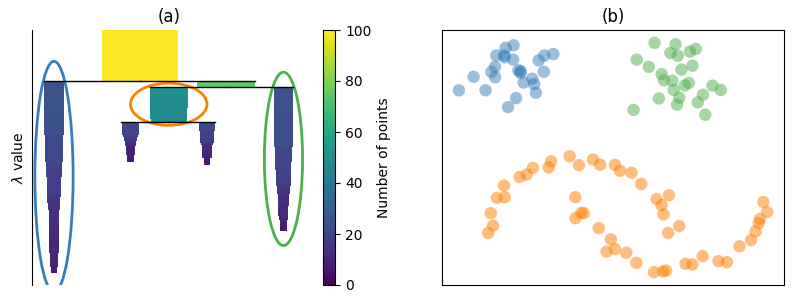
\includegraphics[width=\textwidth]{hdbscan-hierarchy-condensed+results.png}
    \caption{(a) Árbol resultante de condensar la jerarquía mostrada en la figura~\ref{img:hdbscan-hierarchy} usando un tamaño de cluster mínimo de 5 puntos. (b) Resultado del algoritmo sobre el conjunto de datos de la figura~\ref{img:hdbscan-dataset+mst}a.
    Los clusters de mayor estabilidad aparecen seleccionados.}
    \label{img:hdbscan-hierarchy-condensed+results}
\end{figure}

El último paso consiste en extraer la partición de los clusters a partir del árbol condensado.
Con este propósito, HDBSCAN define un criterio para seleccionar aquellos clusters que persisten por más tiempo en la jerarquía.

Como medida alternativa al peso de las aristas (distancia de alcanzabilidad mutua), se define $\lambda=\frac{1}{distancia}$.
Asociamos a cada cluster los valores $\lambda_{birth}$ y $\lambda_{death}$, los valores de $\lambda$ en que surge el cluster y se divide respectivamente.
Y para cada punto $p$ definimos $\lambda_p$ como el valor de $\lambda$ en que $p$ es eliminado de su cluster.
Luego, computamos la \textbf{estabilidad} de un cluster como:

\[
    \sum_{p\in cluster}{\lambda_p - \lambda_{birth}}
\]

Finalmente, inicializamos un conjunto de clusters seleccionados con las hojas del árbol condensado y recorremos el árbol en orden topológico aplicando el siguiente criterio:
Si la suma de la estabilidad de los hijos es mayor que la estabilidad del cluster actual, sustituimos este valor por dicha suma.
Si, por el contrario, la estabilidad del cluster es mayor que la suma de las de sus hijos entonces lo añadimos al conjunto de clusters seleccionados y eliminamos de este a sus descendientes.
Una vez alcanzado el nodo raíz, el algoritmo ha concluido y su resultado son los clusters que hayan quedado en el conjunto.

Cualquier punto que no forme parte de los clusters seleccionados será considerado ruido.
Además HDBSCAN permite, debido al funcionamiento del algoritmo, establecer un valor de pertenencia de los puntos a sus respectivos clusters, normalizando los $\lambda_p$.

% TODO Add HDBSCAN time and space complexity?